A digital twin is a representation of a physical thing, process, or service in digital form. A digital twin is a computer representation of a real thing, such as a jet engine or wind farm, or even larger objects, such as skyscrapers or entire towns. The digital twin technology can be used to reproduce processes in order to collect data and anticipate how they will perform, in addition to real assets.
A digital twin is a computer program that creates simulations based on real-world data to forecast how a product or process will perform. To improve the output, these applications can use the internet of things (Industry 4.0), artificial intelligence, and software analytics. These virtual models have become a standard in modern engineering to drive innovation and enhance performance, thanks to advancements in machine learning and elements such as big data. In brief, having one can help improve strategic technological trends, prevent costly breakdowns in physical objects, and test processes and services utilizing superior analytical, monitoring, and predictive capabilities.
The development of a mathematical model that simulates the original begins with professionals in applied mathematics or data science examining the physics and operational data of a physical object or system. The creators of digital twins make certain that the virtual computer model may get feedback from sensors that collect data from the real-world version. This allows the digital version to mimic and emulate what is happening with the original version in real-time, allowing for the collection of data on performance and potential issues.
A digital twin can be as complicated or as basic as you need it to be, with the quantity of data used deciding how closely the model mimics the actual version in the real world.
The twin can be used in conjunction with a prototype to provide feedback on the product as it is being created, or it can be used as a prototype in and of itself to simulate what might happen when the real version is built.

\begin{figure}
    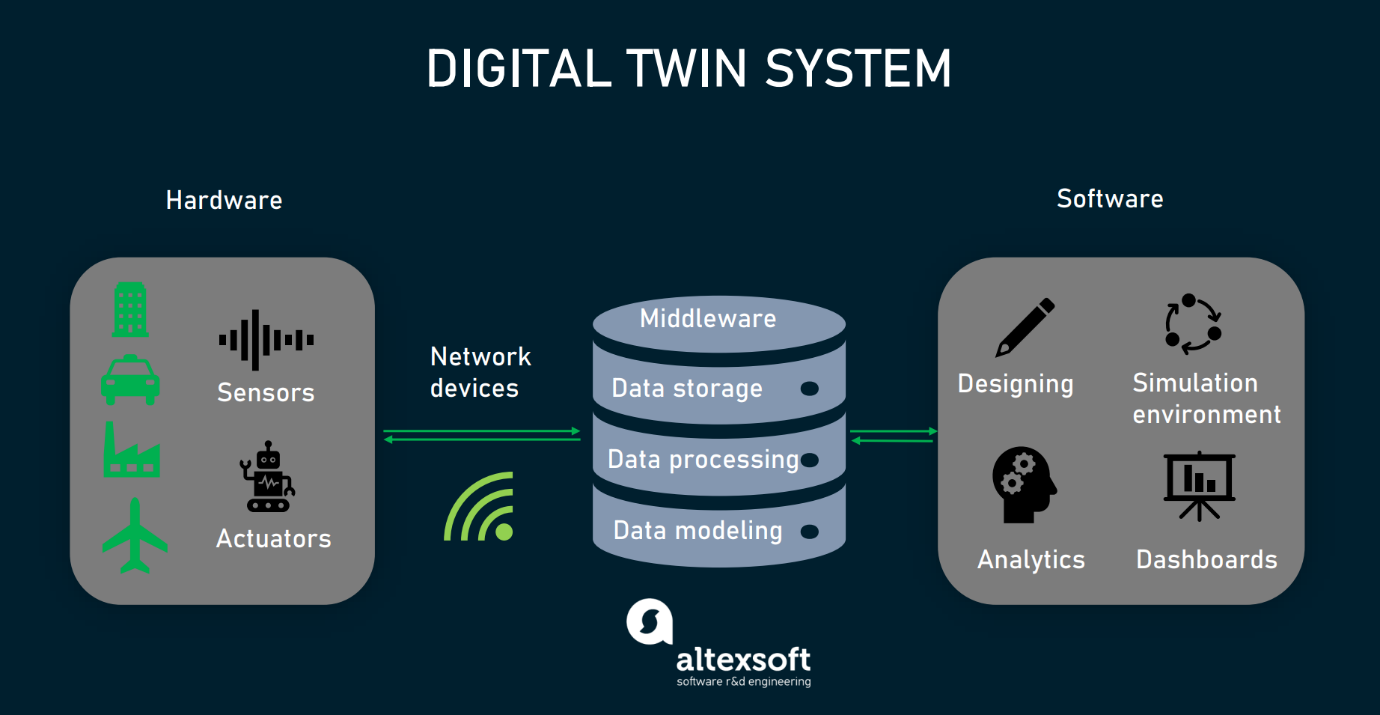
\includegraphics[width=\linewidth]{images/DigitalTwinSystem.png}
    \caption{Components of a Digital Twin.}
    \label{fig:digtaltwinsystem}
  \end{figure}
 
\subsection{Background Knowlege of Digital Twins}
You must first comprehend what you are attempting to construct when creating a Digital Twin. When creating a digital twin of a water plant or a power plant, for example, you'll need to understand how the facility works in real life. To run analytics on that plant, you'll need to gather information about it. Companies will make it difficult for you to obtain data because exposing the info to the public could be dangerous. Let's say you obtained the information by obtaining permission or collecting it yourself or with the help of coworkers. You must be aware of the variables, qualities, and influences on plant changes. You must ask yourself this question. What we want to foretell or what we need to forecast is the question you must now ask yourself. We can start building our digital twin after we know what our goals are and have a good understanding of our data. I've included some questions below that may assist you in asking the right questions as you begin to develop your digital twin.

% generate list
\begin{itemize}
    \item	Do we understand our dataset?
    \item	Is our data useful to make predictions?
    \item	Does our dataset have outliers? Yes, then the software should flag/alert outliers or remove them. When running predictions?
    \item	What behavior are we trying to predict or forecast?
    \item	Are there any relationships in our dataset’s parameters/variables?
    \item	What machine learning methods are we going to use to run analytics/predictions?
\end{itemize}
    
\subsection{Aim of this study and motivation}
If you look at organizations that offer or construct Digital Twin software, you'll see that they charge tens of thousands of dollars to build these solutions. A corporation approached me and told me about the plant's digital twin problem statement. I promised them I could build it for hundreds of dollars in a few weeks. There aren't a lot of resources available on digital twins. I'm filling in the blanks with my experience and knowledge from a solid background in Data Science, Mathematics, and Computer Science. This paper is intended to inspire you to make your businesses smarter and more inventive. It is the fourth Industrial Revolution, and it is time for a shift. The goal of this research is to teach you how to create digital twins. The process for creating digital twins and the knowledge I gained on my own while creating a digital twin of a plant with no prior understanding of digital twins but a background in statistics, data science, and machine learning.

\subsection{Prerequisites}
\begin{itemize}
    \item You will need to have a good understanding of a good statistical/data science language example Python or R
    \item Understanding of statistics and mathematics (if creating custom machine learning models or neural networks) for optimizing machine learning models
    \item Experience in Web Frameworks (used for creating Web Dashboards), Machine Learning Modules (required to forecast and predict data), and a graphing library (MATLAB, Seaborn, etc)
\end{itemize}